\documentclass[12pt,a4paper]{book}

\usepackage[margin=3cm]{geometry}
\usepackage[frenchb]{babel}
\usepackage[utf8]{inputenc}
\usepackage[T1]{fontenc}
\usepackage{graphicx}
\usepackage{url}
\usepackage[colorlinks=true, bookmarks=true, pdfstartview=FitV, linkcolor=blue,citecolor=blue, urlcolor=blue]{hyperref}
\usepackage{lmodern}
\usepackage{fancyhdr}
\usepackage{eurosym}
%\usepackage{color}
\usepackage{makeidx}
\usepackage{epstopdf}
%\usepackage{multicol}
%\usepackage{subfig}
\usepackage{float}
\usepackage{lipsum}

%Pour la frime ;-)
\fancyfoot[LE,RO]{Ce document à été écrit en \LaTeX}

%\usepackage{listings} %basic greyed code highlighting package
\usepackage{texments} %code highlighting package
\usestyle{colorful}

\title{Rapport de stage TN09}
\author{Paul Grandperrin}
\date{du 5 septembre au 17 février 2012}
\makeindex
\pagestyle{fancy}
\begin{document}

\maketitle
\tableofcontents

\frontmatter



\part{Introduction}
\chapter{L'entreprise}
\section{Alter Way}
\paragraph*{}
	Alter Way est une entreprise spécialisée dans les services {\bf open source}. Elle est composée
	de cinq groupes afin de répondre à l'ensemble des besoins des SI\footnote{Système d'Information}:
	\begin{description}
		\item[Hosting] Hébergement et infogérance système de site web
		\item[Solution] Développent, maintenance et infogérance applicatif de site web
		\item[Formation] Formation standard, cursus de formation, coatching
		\item[Consulting] Conseil, audit, industrialisation
		\item[Creative] Conseil en communication, infographisme
	\end{description}

	\begin{figure}
	\centering
	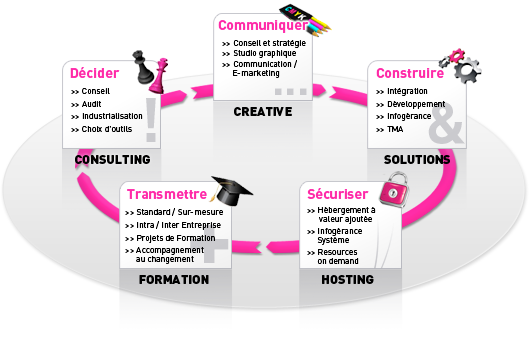
\includegraphics[width=0.9\textwidth]{img/aw_360}
	\caption{Les différentes branches d'Alter Way}
	\end{figure}

\section{Histoire}
\paragraph*{}
	Créee en 2006, Alter Way est la première entreprise française à avoir fédéré les acteurs historique
	de l'open source autour d'un projet d'industrialisation du marché:

	\begin{description}
		\item[Anaska] Leader français de formation open source en 2001
		\item[Eclip's Software] Éditreur d'une solution d'administration réseau
		\item[Ingeniweb] Spécialiste en solution web d'entreprise de gestion de contenu
		\item[Kanopee] Consultants en développement PHP
		\item[Nexen Services] Hébergement et Infogérance LAMP\footnote{Linux Apache MySQL PHP}
		\item[O4DB] Expertise en BDD\footnote{Base de Donnée}
		\item[Solinux] Spécialistes dans l'administration de platforme Linux et l'intégration d'OpenXchange
	\end{description}

	Afin de renforcer son offre globale et de soutenir sa stratégie de développement sur le web, Alter Way
	a également intégré l'agence de communication {\bf Reciprok}, spécialisée en conseil en communication,
	studio graphique et web-marketing.

	\begin{figure}
	\centering
	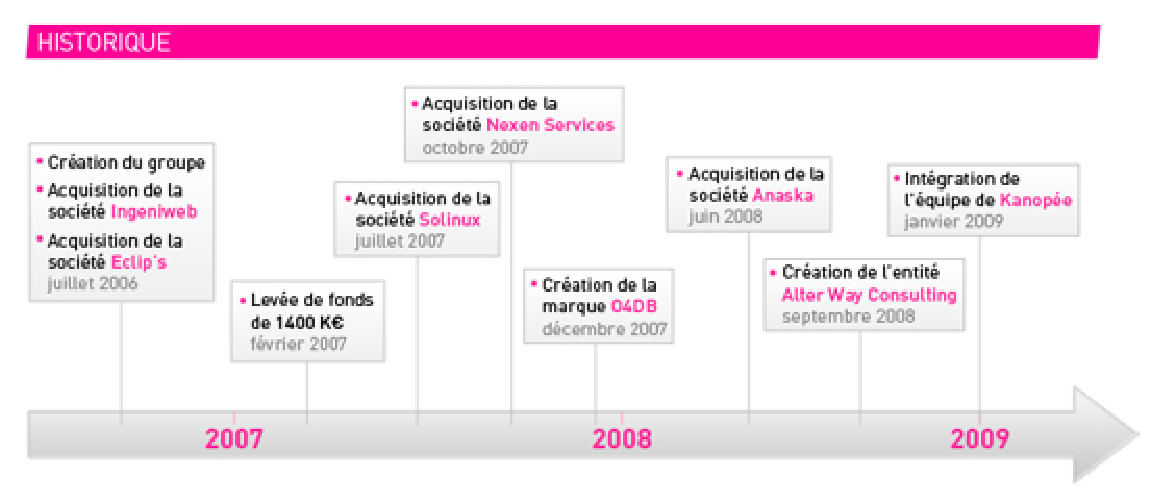
\includegraphics[width=0.9\textwidth]{img/historique_aw}
	\caption{L'histoire d'Alter Way}
	\end{figure}

\section{Quelques chiffres (2010)}
	\begin{itemize}
		\item 10M\euro{} de Chiffre d'affaire
		\item 10\% de croissance
		\item Résultats: +4.5\%
		\item 120 collaborateurs
	\end{itemize}


\section{Alter Way Hosting}
\paragraph*{}



\mainmatter
\part{Déroulement du stage}

\paragraph*{}
\lipsum[1]


\chapter{Projet OpenNebula}

\section{Premiers pas}

\paragraph*{}
Les premiers jours de mon stage ont été dédiés pour tester les logiciels OpenNebula et Xen sur une platforme de test
composée d'un petit serveur accueillant OpenNebula, de deux machines utilisées comme hyperviseurs Xen et d'un NetApp.
Vivien, pour responsable de stage, avait déjà déployé un environnement de développement fonctionnel sur ces machines.

\paragraph*{}
Afin de prendre en main la platforme, mon premier objectif à été de mettre à jour OpenNebula qui était en version 2.2 vers la version 3.0 Beta 1.
Cette version 2.2 a été modifié par Vivien pour fonctionner avec un plugin qu'il a écrit pour ajouter le support de l'iSCSI pour déporter le stockages des images
disque des VMs sur le NetApp.
\\
Il m'a donc fallu comprendre puis adapter le travail de Vivien. J'ai ensuite effectué beaucoup de tests pour valider le fonctionnement
de la nouvelle solution et aussi en valider ma compréhension.
\\
Après avoir compris comment marchait OpenNebula de l'extérieur - en tant qu'utilisateur - j'ai téléchargé les sources et ai préparé un
environnement de développement pour éditer, compiler\footnote{Étape de construction de l'exécutable du logiciel à partir des sources},
débugger\footnote{Action de compiler et lancer un exécutable d'une certaine manière permettant de voir le fonctionnement interne de l'application
pendant son fonctionnement pour comprendre et corriger des bugs}, installer et tester le logiciel.

\section{Interface de commande}
\paragraph*{}
OpenNebula peut être piloté via plusieurs interfaces:
\begin{listi}
	\item une interface web appelé Sunstone. voir figure \ref{sunstone}.
	\item une CLI\footnote{\index{CLI}CLI: \emph{Command Line Interface}, interface en ligne de commande}. voir \ref{clione}.
	\item une API\footnote{\index{API}API: \emph{Application Programming Interface}, Interface de programmation} de type
		XML\footnote{XML: \emph{Extensible Markup Language}, langage de balisage extensible, est un format de de structuration de donnée générique.}/RPC
		\footnote{RPC: \emph{Remote Procedure Call}, appel de procédure distant, est un protocole réseau fait pour appeler des procédure au sein d'un programme
		travers d'un réseau}
\end{listi}

\subsection{La CLI d'OpenNebula}
\label{onecli}

\subsubsection{L'affichage de la liste de tout les \emph{hosts}/hyperviseurs}
\begin{lstlisting}
oneadmin@opennebula:~$ onehost list
  ID NAME               RVM   TCPU   FCPU   ACPU   TMEM   FMEM   AMEM   STAT
   0 hyp1                 1    400    399    300     4G   2.7G   3.9G     on
   1 hyp2                 2    400    399    100     4G   1.2G   3.2G     on
\end{lstlisting}

\subsubsection{L'affichage de la liste des VMs}
\begin{lstlisting}
oneadmin@opennebula:~$ onevm list
ID USER     GROUP    NAME         STAT CPU     MEM        HOSTNAME        TIME
 0 oneadmin oneadmin vm1          runn   1    256M            hyp2 08 03:36:24
 1 oneadmin oneadmin vm2          runn   4   2048M            hyp2 00 00:01:38
 2 oneadmin oneadmin vm3          runn   2    128M            hyp1 00 00:01:00
\end{lstlisting}

\subsection{L'interface web Sunstone}

\begin{figure}[H]
\centering
\subfloat[\emph{Dashboard} / Tableau de bord]{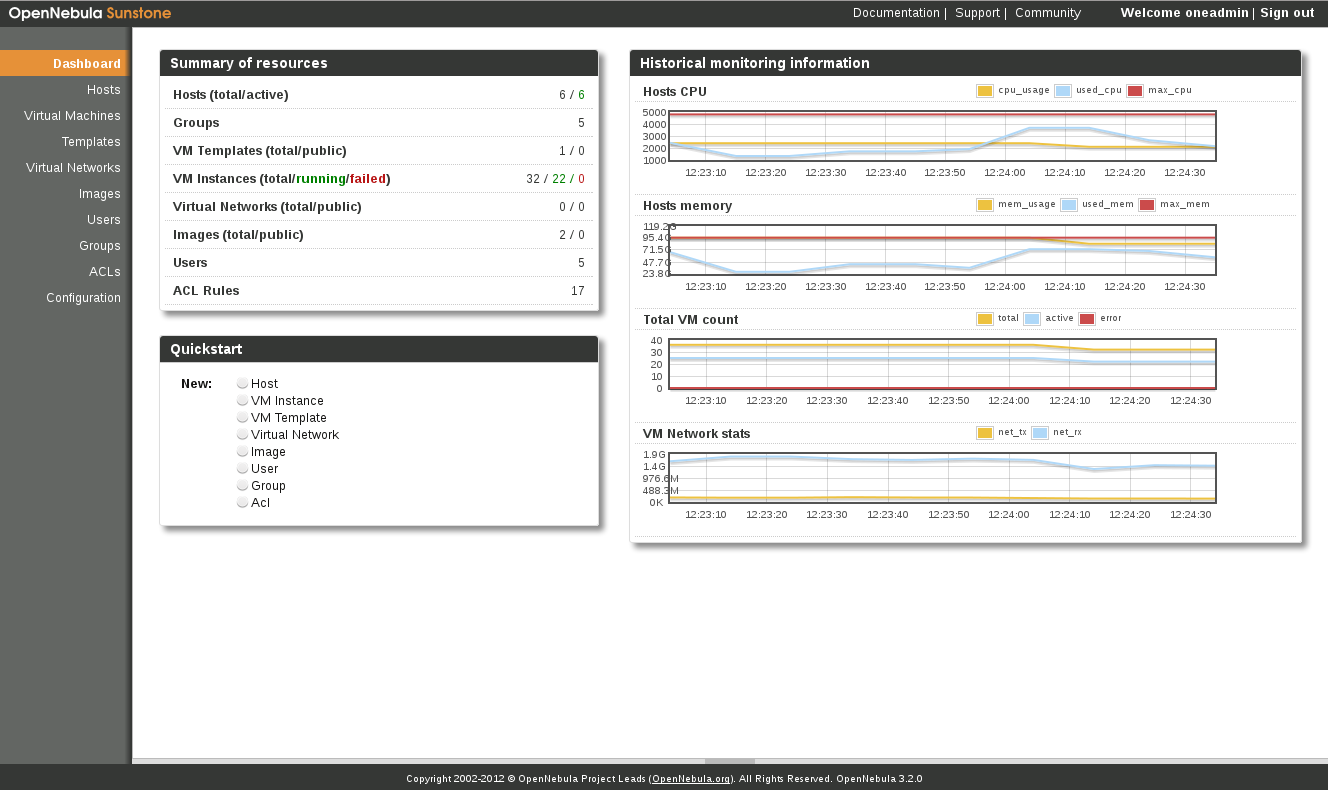
\includegraphics[width=0.5\textwidth]{resource/img/sunstone-dashboard}}
\subfloat[Création d'une VM]{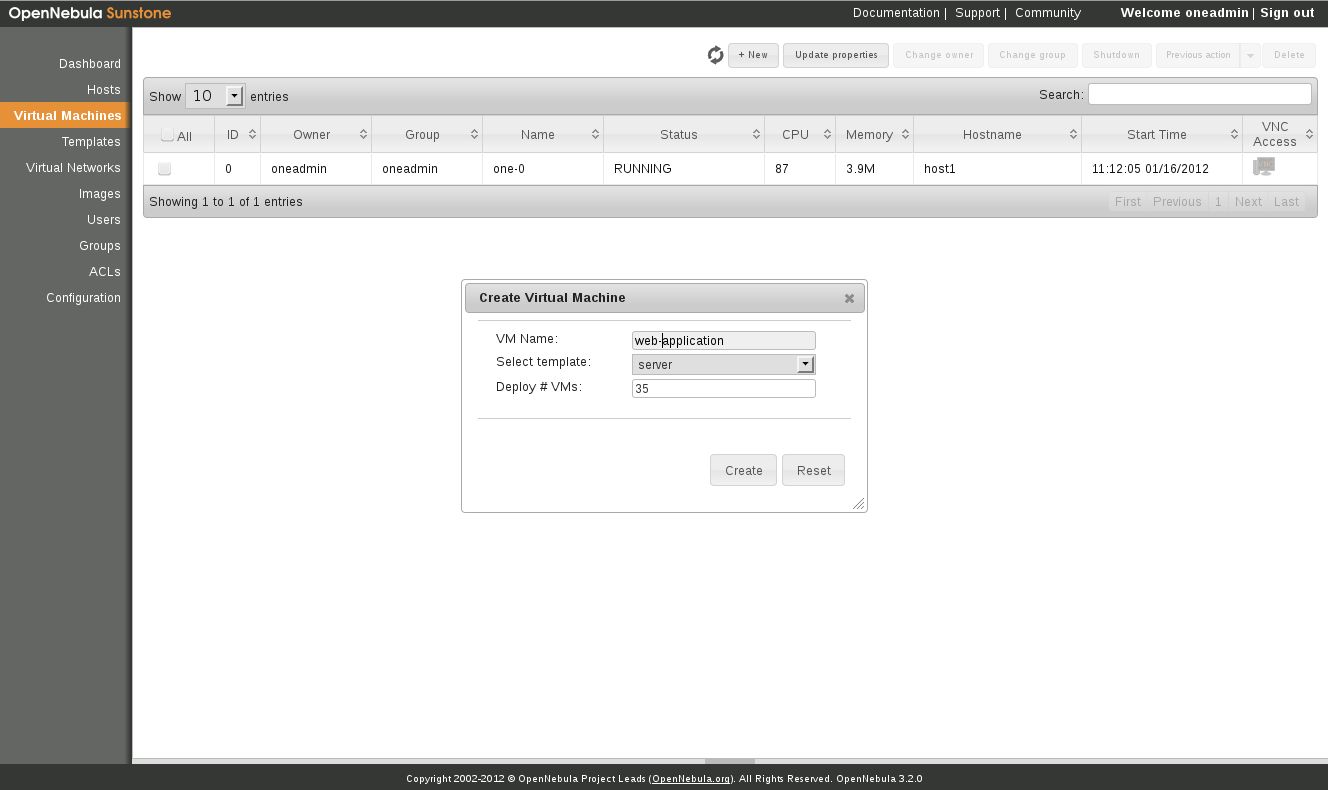
\includegraphics[width=0.5\textwidth]{resource/img/sunstone-createvm}}
\\
\subfloat[Création d'un template de VM]{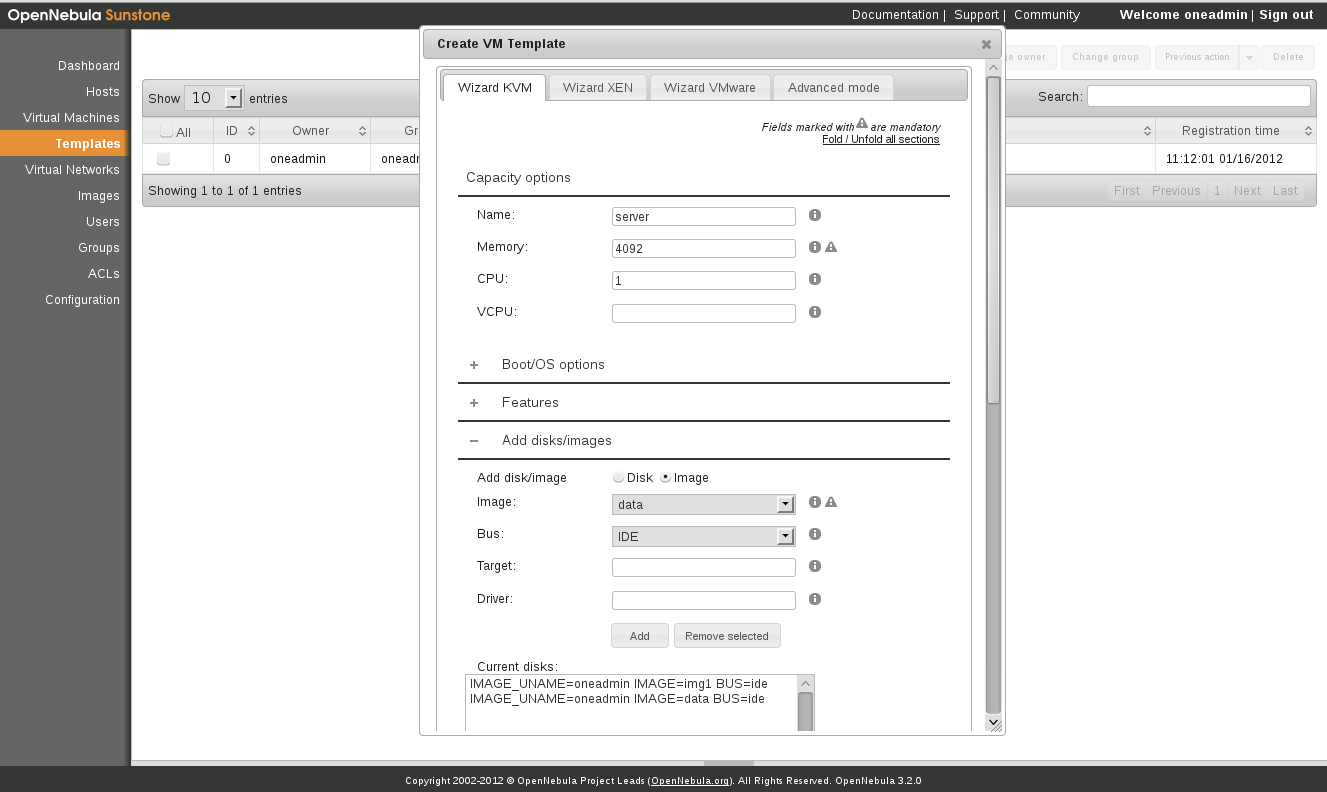
\includegraphics[width=0.5\textwidth]{resource/img/sunstone-createtemplate}}
\subfloat[Affichage de la liste des \emph{hosts}]{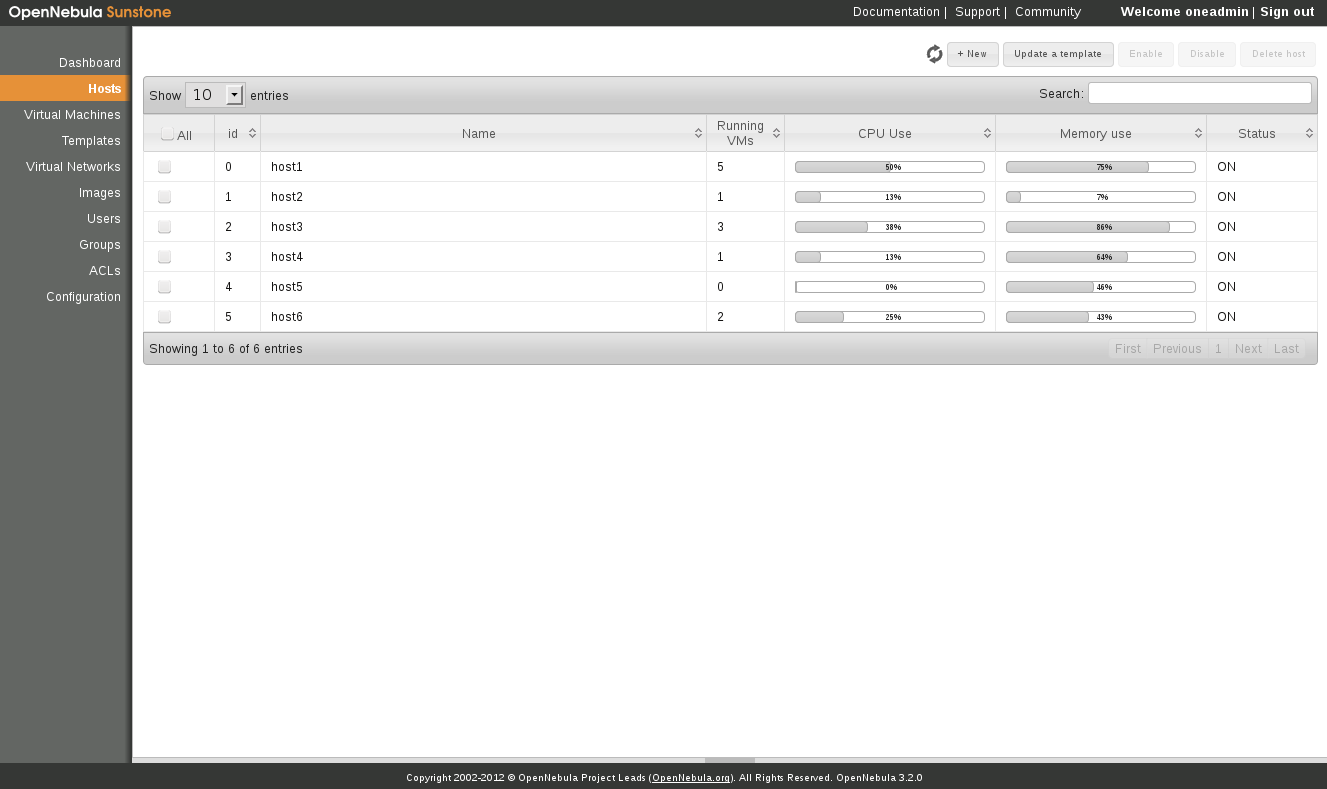
\includegraphics[width=0.5\textwidth]{resource/img/sunstone-hosts}}

\caption{L'interface web Sunstone d'OpenNebula}
\index{Sunstone}
\label{sunstone}
\end{figure}

\subsection{Architecture du code d'OpenNebula}
\paragraph*{}
Le code d'OpenNebula est designé comme une machine à état séparés en modules qui communiquent des ordres d'action de manière asynchrone.
\\
Chaques modules tourne dans le contexte d'un \emph{thread} et utilise une file d'attente FIFO\footnote{FIFO: \emph{First In First Out}, est une structure de donnée où les données poussées à l'interieur
en premier sont celles qui en sortent en premier aussi} pour recevoir les messages des autres \emph{threads} de manière asynchrone.

\paragraph*{}
La machine à état d'OpenNebula est principalement axé autour des états des VMs et plus précisément autour du lien entre les VMs et les \emph{Hosts}.


\section{L'environnement}

\paragraph*{}
Pour l'ajout des fonctions de \emph{scale-in}, j'ai du en même temps regarder ce qui était techniquement possible au niveau de l'hyperviseur Xen qui
sera utilisé comme backend\footnote{Un backend est la partie basse d'une architecture utilisé pour éffectuer des actions à l'extérieur du logiciel.
Par opposition le frontend est la partie haute de l'architecture recevant les ordres de l'utilisateur et commandant les autres parties de l'architecture}
par OpenNebula pour crééer les VMs sur un hyperviseur.

\paragraph*{}
En effet, en fonction des différentes version du noyau Linux et de Xen, certaines fonctionnalités sont disponibles, indisponibles ou buggés.\\
J'ai donc fait un tableau LibreOffice Calc\footnote{Logiciel open source concurrent de Microsoft\textsuperscript{\textregistered} Excel\texttrademark}
pour répertorier l'état de chaques fonctionnalités en fonction de toutes les combinaisons de versions possibles.
\\
Grâce à ce tableau, nous avons pu déterminer quelles étaient les fonctionnalités nous utiliserons et par déduction quelles versions de logiciels nous
installerons.

\paragraph*{}
Après avoir expérimenté avec la base de code d'OpenNebula nous avons fait des dessins d'architecture et une déterminé une procedure pour mettre en oeuvre ces
modifications.


\section{Nouvelle architecture}

L'objectif était de commencer par s'occuper des modifications de la gestion du stockage puis d'ajouter le support du \emph{scale in} qui est moins important.

\subsection{La gestion du stockage des images disque}
\paragraph*{}
Pour l'instant OpenNebula considère que les images disque des VMs sont soit stockées en local sur l'hyperviseur soit partagées sur un répertoire NFS
	\footnote{NFS: Network File System, est un système de fichier qui permet d'accèder à des fichiers via le réseau. Plusieurs clients peuvent accèder
	au mêmes fichiers en même temps. Ce système ressemble au protocole SMB de Microsoft\textsuperscript{\textregistered}}\index{NFS}
.
Vivien à aussi écrit un plugin OpenNebula pour partager les images disque via l'iSCSI - plus performant que le NFS pour ce type d'utilisation.
\\
Dans tout les cas, OpenNebula n'a pas été designé pour gérer plusieurs serveurs de stockage et répartir les images disque dessus.
\\
Les deux objets les plus important manipulés par OpenNebula sont les \emph{Hosts} et les VMs. Un \emph{Host} est le nom utilisé par OpenNebula pour
désigner un hyperviseur.
Un \emph{Host} contient donc zéro ou plusieurs VMs et une VM a forcément un et un seul \emph{Host} associé.


\paragraph*{}
Notre objectif serait de faire la même relation entre les images disques vs les serveurs de stockage et les VMs vs les \emph{Hosts}.
\\
OpenNebula n'a pour l'instant pas la notion de ce qu'est un serveur de stockage. Une image disque est juste un attribut d'une VM et n'a
pas de propriété faite pour désigner sur quel serveur de stockage elle se trouve.\\
De plus, par défault, OpenNebula considère que l'image disque d'une VM ne contient aucune donnée importante et est supprimée aussitôt
que la VM est détruite.

\paragraph*{}
Nous avons donc créé dans le code d'OpenNebula un nouveau type d'objet appelé \emph{storage backend}, littéralement << object s'occupant du stockage >>.
Un \emph{storage backend} pourra être un NetApp, un serveur NFS ou un cluster Ceph par exemple. Une image disque devient donc principalement un attribut d'un
\emph{storage backend} et peut vivre et être manipulées indépendement des VMs.\\


\paragraph*{}
Ce nouvelle object à nécéssité énormément de modifications au code source d'OpenNebula:
\begin{enumerate}
	\item Ajout de plusieurs modules pour gérer le cycle de vie d'un \emph{storage backend} et ses liens avec les autres objets du système.
	\item Designer un protocole de communication générique avec les driver/pilote des \emph{storage backend}.
	\item L'écriture d'une architecture de gestion de plugin/driver pour communiquer avec le \emph{storage backend} en question.
	\item Rédesigner entièrement et réécrire le \emph{Transfert Manager} (Gestionnaire de transfert) car il n'était pas du tout assez flexible
		pour gérer les tranferts entre différents \emph{storage backend}.
	\item Étendre le protocole XML/RPC et les outils de la CLI pour pouvoir administrer ces nouvelles fonctionnalités.
	\item Documenter les modifications
	\item Écrire des tests unitaires pour vérifier qu'il n'y a pas de régressions introduites.
\end{enumerate}

\section{Bilan}

\paragraph*{}








\chapter{Le projet H2O}



\chapter{Le projet Kanopya}

\section{Présentation}


\chapter{Autres travaux}

\section{Conférence OpenStack}

\section{Projet STERN}


\section{Déployement automatisé de site web Symfony 2}


\section{Déployement de Bacula sur FreeBSD et ZFS}


\begin{pygmented}{c}
void main(int argc, char* argv[])
{
	printf("hello");
	return 0;
}
\end{pygmented}

\cite{test}

\appendix
\part{Annexe}

\chapter{Photos illustratives d'�quipements informatique}

\begin{figure}[H]
	\centering
	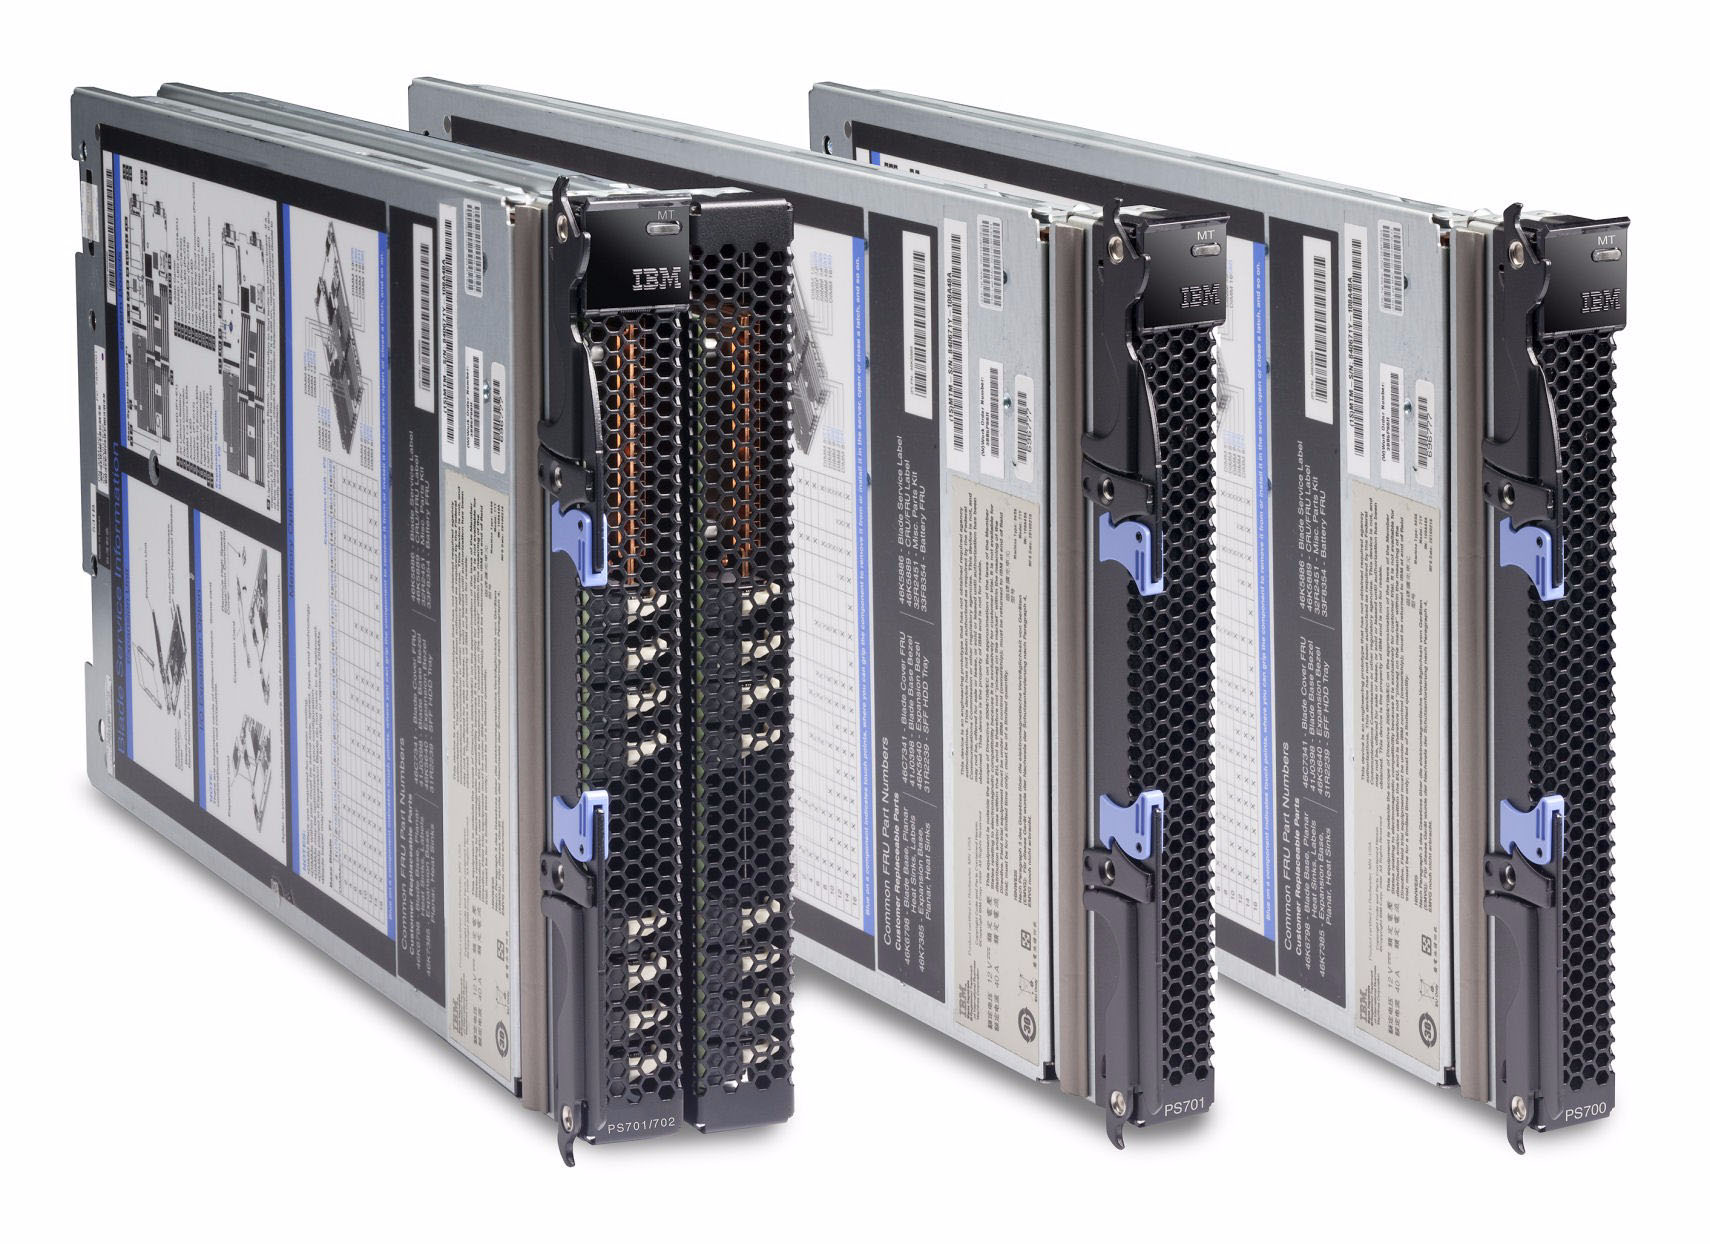
\includegraphics[width=0.6\textwidth]{resource/img/blade}
	\caption{Trois serveurs lames (\emph{blade server} en anglais)}
\end{figure}

\begin{figure}[H]
	\centering
	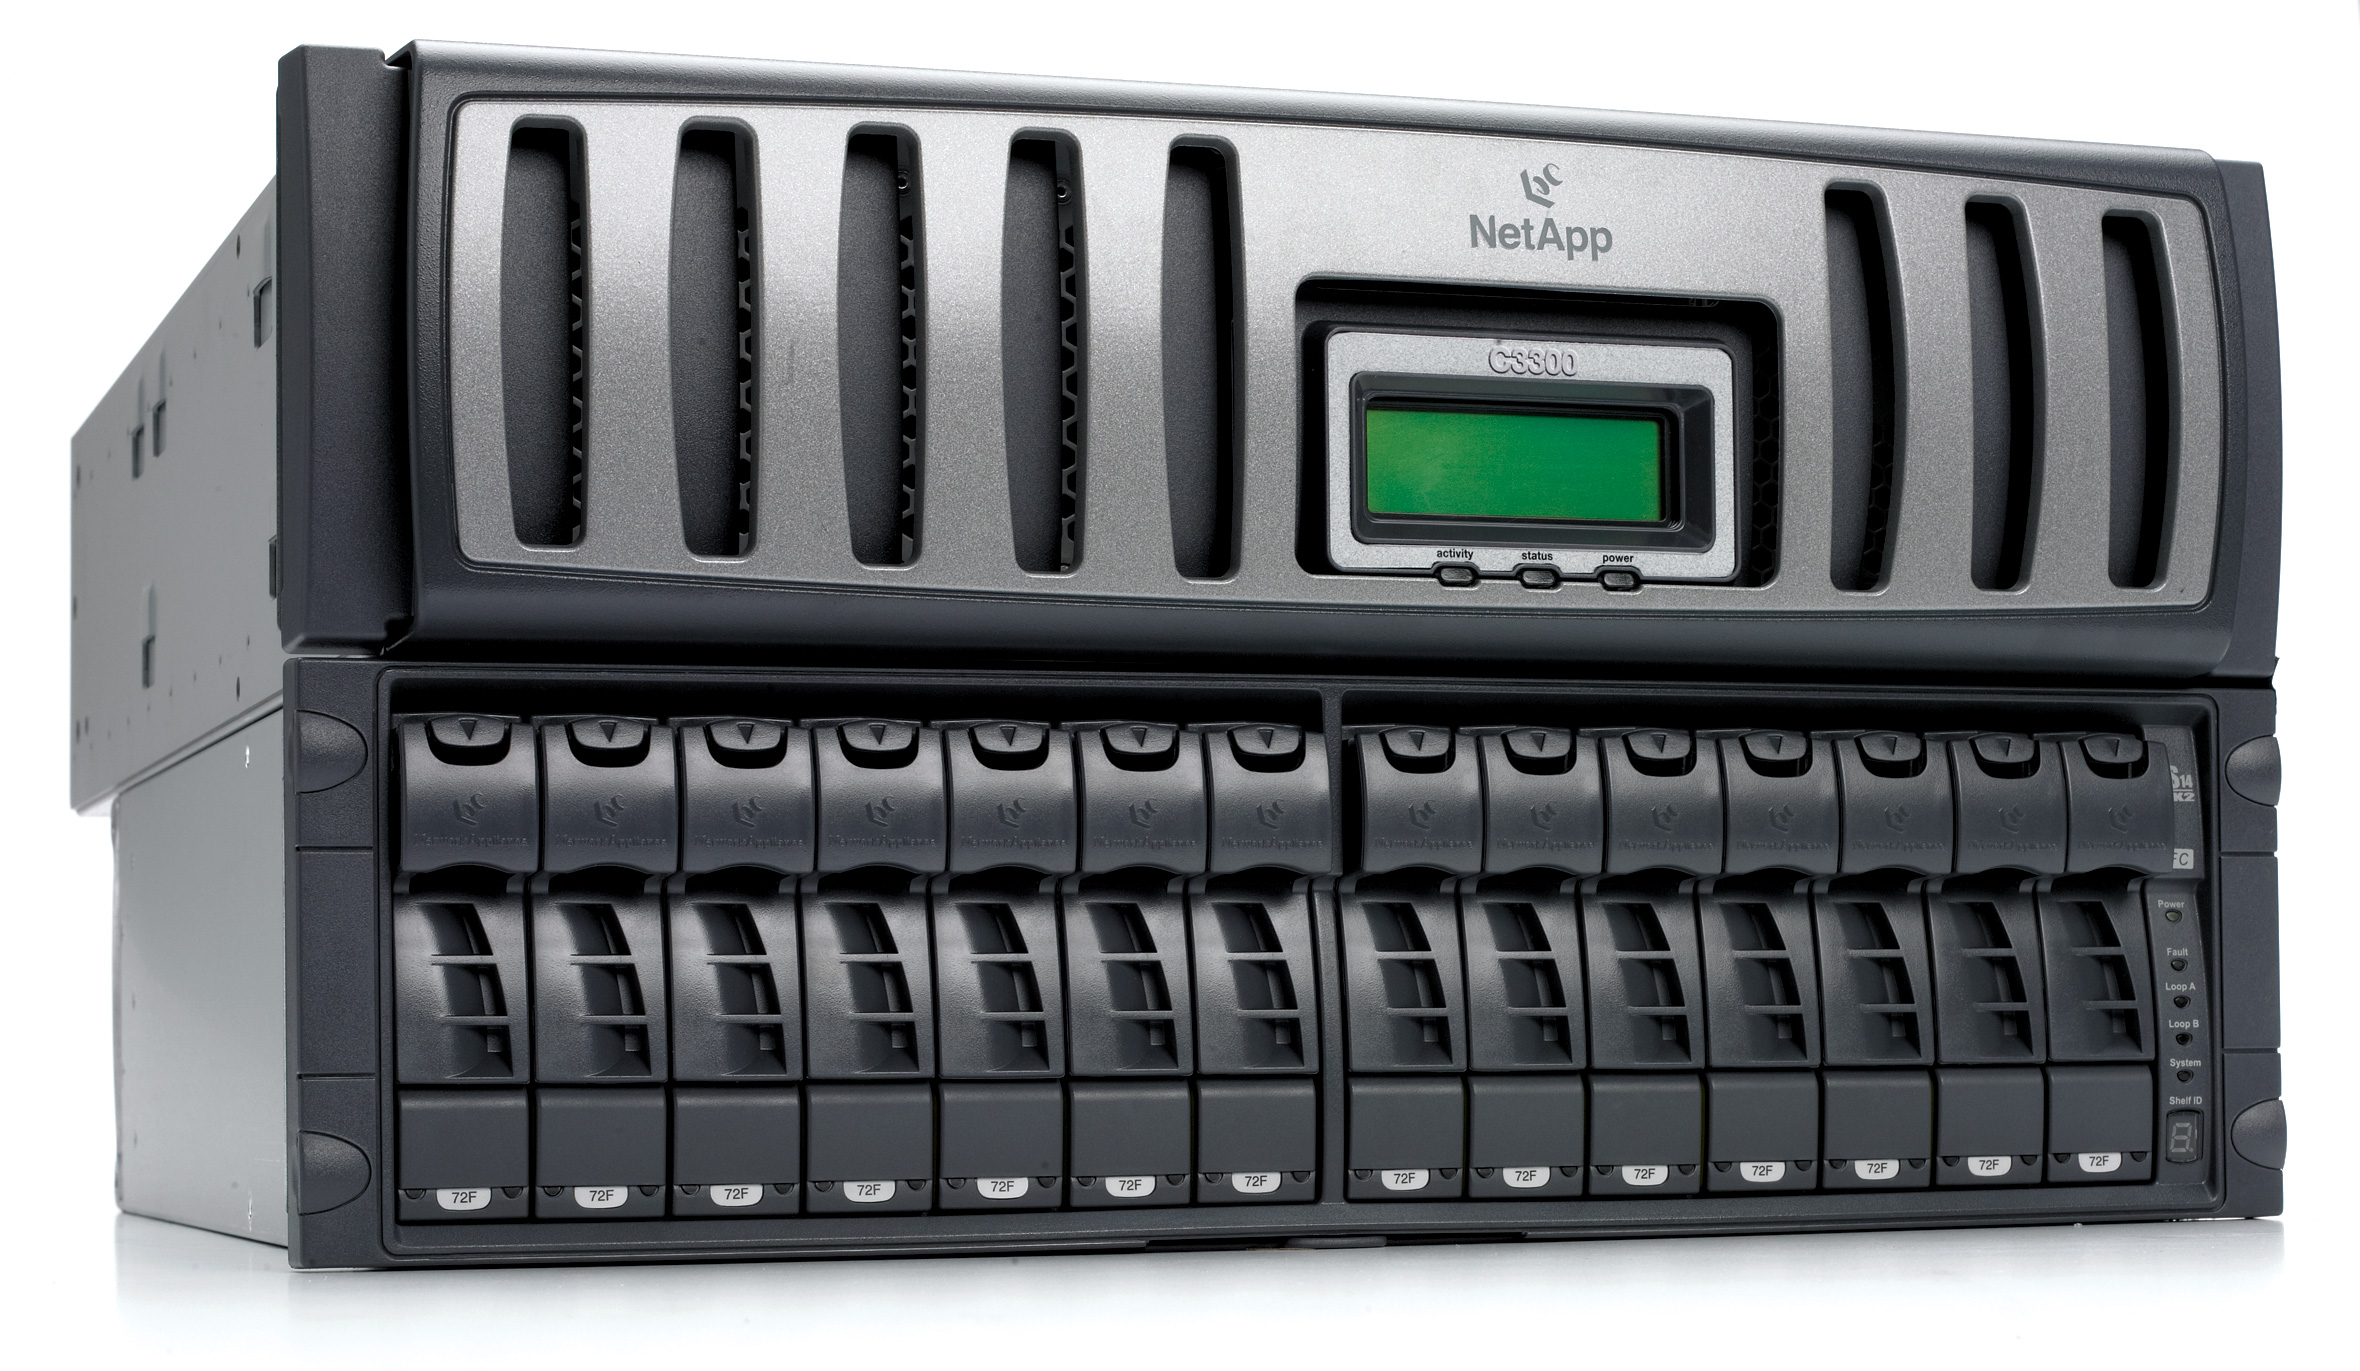
\includegraphics[width=0.6\textwidth]{resource/img/netapp_c3300}
	\caption{Baie de disque NetApp C3300 contenant 14 disques durs}
	\label{netapp}
\end{figure}

\begin{figure}[H]
	\centering
	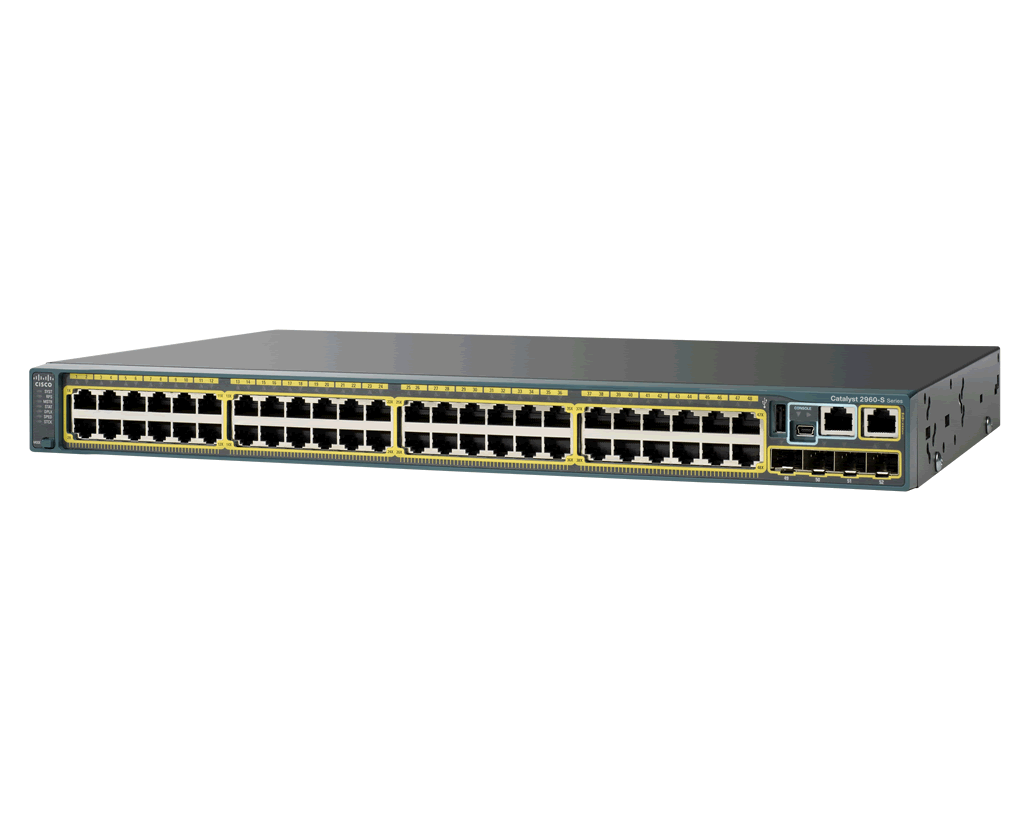
\includegraphics[width=0.6\textwidth]{resource/img/cisco-switch}
	\caption{Switch Cisco WS-C2960}
\end{figure}

\begin{figure}[H]
	\centering
	\includegraphics[width=0.6\textwidth]{resource/img/DC}
	\caption{Plusieurs baies de serveur (\emph{rack} en anglais) dans un Data Center}
	\label{datacenter}
\end{figure}

\chapter{R�sum� des changement apport�s � OpenNebula pour l'ajout de la gestion \emph{storage sackend}}
\label{modopennebula}
\begin{lstlisting}
 SConstruct                                     |    6 +-
 include/AuthManager.h                          |    4 +-
 include/DispatchManager.h                      |   17 ++-
 include/Image.h                                |   18 ++-
 include/ImageManager.h                         |   30 ++--
 include/ImagePool.h                            |    2 +
 include/Nebula.h                               |   26 ++-
 include/RequestManagerAllocate.h               |   39 +++-
 include/RequestManagerDelete.h                 |   18 ++
 include/RequestManagerHost.h                   |   20 ++
 include/RequestManagerImage.h                  |   27 +++
 include/RequestManagerInfo.h                   |   18 ++
 include/RequestManagerPoolInfo.h               |   18 ++
 include/RequestManagerStorageBackend.h         |   59 +++++
 include/RequestManagerUpdateTemplate.h         |   18 ++
 include/StorageBackend.h                       |  184 +++++++++++++++
 include/StorageBackendPool.h                   |   85 +++++++
 include/StorageBackendTemplate.h               |   27 +++
 include/StorageManager.h                       |  155 ++++++++++++
 include/StorageManagerDriver.h                 |   53 +++++
 include/TransferManager.h                      |   46 +++--
 include/TransferManagerDriver.h                |   89 +++++++-
 include/VirtualMachine.h                       |   17 ++-
 install.sh                                     |   34 +++-
 share/etc/oned.conf                            |   33 +++-
 share/man/SConstruct                           |    1 -
 src/acct/watch_helper.rb                       |    6 +-
 src/cli/etc/oneimage.yaml                      |    5 +
 src/cli/etc/onestoragebackend.yaml             |   50 ++++
 src/cli/one_helper.rb                          |    2 +-
 src/cli/one_helper/oneimage_helper.rb          |    8 +-
 src/cli/one_helper/onestoragebackend_helper.rb |  110 +++++++++
 src/cli/oneimage                               |   21 ++
 src/cli/onestoragebackend                      |   98 ++++++++
 src/cloud/common/CloudAuth/EC2CloudAuth.rb     |    2 -
 src/cloud/common/CloudAuth/X509CloudAuth.rb    |    3 +-
 src/dm/DispatchManagerActions.cc               |   47 ++++
 src/image/Image.cc                             |   26 ++-
 src/image/ImageManagerActions.cc               |    6 +
 src/image/ImageManagerDriver.cc                |    1 +
 src/image/ImagePool.cc                         |   37 ++-
 src/lcm/LifeCycleActions.cc                    |    1 +
 src/lcm/LifeCycleStates.cc                     |    2 -
 src/mad/MadManager.cc                          |    1 +
 src/mad/ruby/ActionManager.rb                  |   20 +-
 src/mad/ruby/StorageDriver.rb                  |  101 ++++++++
 src/mad/ruby/TransfertManagerDriver.rb         |  170 ++++++++++++++
 src/nebula/Nebula.cc                           |   31 +++-
 src/nebula/SConstruct                          |    2 +
 src/oca/ruby/OpenNebula.rb                     |    2 +
 src/oca/ruby/OpenNebula/Image.rb               |   12 +-
 src/oca/ruby/OpenNebula/Pool.rb                |   11 +-
 src/oca/ruby/OpenNebula/StorageBackend.rb      |  127 ++++++++++
 src/oca/ruby/OpenNebula/StorageBackendPool.rb  |   53 +++++
 src/oca/ruby/OpenNebula/XMLUtils.rb            |    1 -
 src/onedb/onedb                                |    6 +-
 src/onedb/onedb_backend.rb                     |   18 +-
 src/rm/Request.cc                              |    2 +
 src/rm/RequestManager.cc                       |   24 ++-
 src/rm/RequestManagerAllocate.cc               |   16 ++
 src/rm/RequestManagerImage.cc                  |   88 +++++++
 src/rm/RequestManagerStorageBackend.cc         |   69 ++++++
 src/rm/RequestManagerVirtualMachine.cc         |   18 ++-
 src/rm/SConstruct                              |    1 +
 src/sm/SConstruct                              |   12 +
 src/sm/StorageManager.cc                       |  298 ++++++++++++++++++++++++
 src/sm/StorageManagerDriver.cc                 |  228 ++++++++++++++++++
 src/sm_mad/dummy/one_sm_dummy                  |   37 +++
 src/sm_mad/dummy/one_sm_dummy.rb               |   42 ++++
 src/storagebackend/SConstruct                  |   12 +
 src/storagebackend/StorageBackend.cc           |  256 ++++++++++++++++++++
 src/storagebackend/StorageBackendPool.cc       |   87 +++++++
 src/storagebackend/test/SConstruct             |    1 +
 src/test/Nebula.cc                             |    1 +
 src/tm/TransferManager.cc                      |  131 ++++++-----
 src/tm/TransferManagerDriver.cc                |  156 ++++++++++++-
 src/tm_mad/dummy/one_tm_dummy                  |   37 +++
 src/tm_mad/dummy/one_tm_dummy.rb               |   43 ++++
 src/tm_mad/dummy/tm_dummy.conf                 |   23 --
 src/tm_mad/dummy/tm_dummy.sh                   |   19 --
 src/tm_mad/dummy/tm_dummyrc                    |   15 --
 src/tm_mad/lvm/tm_context.sh                   |    9 +-
 src/tm_mad/lvm/tm_lvmrc                        |    3 -
 src/tm_mad/shared/tm_context.sh                |   10 +-
 src/tm_mad/shared/tm_sharedrc                  |    4 -
 src/tm_mad/ssh/tm_context.sh                   |   10 +-
 src/tm_mad/ssh/tm_mv.sh                        |   17 +-
 src/tm_mad/ssh/tm_sshrc                        |    4 -
 src/tm_mad/tm_common.sh                        |   14 --
 src/vm/VirtualMachine.cc                       |    4 +
 src/vm/VirtualMachinePool.cc                   |   55 +++++
 91 files changed, 3471 insertions(+), 299 deletions(-)
\end{lstlisting}

\chapter{H2O}

\section{R�sum� du code d�velopp�}

\begin{lstlisting}
 bin/h2o-archive            |  181 +++++++++++++
 bin/h2o-block              |  392 +++++++++++++++++++++++++++
 bin/h2o-cluster            |  598 +++++++++++++++++++++++++++++++++++++++++
 bin/h2o-loader             |  186 +++++++++++++
 bin/h2o-setup-db           |   22 ++
 bin/h2o-vif                |  235 ++++++++++++++++
 bin/h2o-vm                 |  529 ++++++++++++++++++++++++++++++++++++
 bin/h2ocheck               |  143 ++++++++++
 bin/h2od                   |   94 +++++++
 conf.rb                    |   11 +
 lib/cli.rb                 |  332 +++++++++++++++++++++++
 lib/dm-options.rb          |   35 +++
 lib/errors.rb              |   16 ++
 lib/lockable.rb            |   16 ++
 lib/logging.rb             |   11 +
 lib/manageable.rb          |  185 +++++++++++++
 lib/manager.rb             |   52 ++++
 lib/modules.rb             |    5 +
 lib/sshtarget.rb           |  109 ++++++++
 lib/tagable.rb             |   64 +++++
 managers/archive.rb        |   84 ++++++
 managers/block-pool.rb     |  130 +++++++++
 managers/block.rb          |  142 ++++++++++
 managers/cluster.rb        |   53 ++++
 managers/hypervisor.rb     |   94 +++++++
 managers/loader.rb         |   41 +++
 managers/vif.rb            |   99 +++++++
 managers/vm.rb             |  640 +++++++++++++++++++++++++++++++++++++++++++
 model/vm.rb                |  642 ++++++++++++++++++++++++++++++++++++++++++++
 modules/dummyblockpool.rb  |   66 +++++
 modules/dummyhypervisor.rb |   42 +++
 modules/netapp.rb          |  379 ++++++++++++++++++++++++++
 modules/xenhypervisor.rb   |  397 +++++++++++++++++++++++++++
 remote/attach-block.sh     |    3 +
 remote/pack.sh             |   23 ++
 remote/unpack.sh           |   31 +++
 templates/xmdomain.erb     |   21 ++
 tests/check.sh             |   52 ++++
 tests/cleanup-netapp.sh    |   10 +
 tests/dropshell.sh         |    4 +
 tests/reset-archivepool.sh |    4 +
 tests/reset-hyp.sh         |   10 +
 tests/reset-master.sh      |    4 +
 tests/reset-netapp.sh      |   12 +
 tests/vm-lifecycle.sh      |   59 ++++
 45 files changed, 6258 insertions(+), 0 deletions(-)
\end{lstlisting}

\section{La \emph{Command Line Interface}}
\label{CLIH2O}
\subsection{Interface de gestion de cluster}

\begin{lstlisting}
paulg@debian-pro:~/projects/h2o$ ./bin/h2o-cluster list
=>Argument Error<=
The first argument must be an action


Possible actions:
        register-hyp <cluster-id> <driver> <hostname> <ssh-user> <ssh-host>
        register-blockpool <cluster-id> <driver> <name> <target-ip> <management-ip> <management-user>
        register-cluster <name> <archive_pool_ip> <archive_pool_user>
        list-hyp [--cluster <id>] [--show-destroyed]
        list-blockpool [--cluster <id>] [--show-destroyed]
        list-cluster [--show-destroyed]
        unregister-hyp <id>
        unregister-blockpool <id>
        unregister-cluster <id>
        lock-cluster <id>
        lock-hyp <id>
        lock-blockpool <id>
        unlock-cluster <id>
        unlock-hyp <id>
        unlock-blockpool <id>
        unload-hypervisor <id>
        clear-error-cluster <id>
        clear-error-hyp <id>
        clear-error-blockpool <id>
        retry-cluster <id>
        retry-hyp <id>
        retry-blockpool <id>
        set-tag-hyp <id> [[+|-]<tag> ...]
        set-tag-blockpool <id> [[+|-]<tag> ...]
        show-hyp <id>
        show-blockpool <id>

Global optional arguments
        --raw : Print results formated for easy scripting
        --override: Disable most checks when trying to do the action
        --force: Will try harder to do the action
        --wait: Wait for the action to finish before returning
\end{lstlisting}

\subsection{Interface de gestion de VMs}

\begin{lstlisting}
paulg@debian-pro:~/projects/h2o$ ./bin/h2o-vm
=>Argument Error<=
The first argument must be an action


Possible actions:
        create <clusterId> <name>
        destroy <id>
        start <id>
        halt <id>
        reboot <id>
        mem-set <id> <size> #The memory size is in megabytes
        maxmem-set <id> <size> #The max memory size is in megabytes
        vcpu-set <id> <vcpu count>
        maxvcpu-set <id> <max vcpu count>
        show <id>
        list [--cluster <clusterId>] [--hyp <hypId>] [--show-destroyed]
        livemigrate <id> <hypervisorId>
        attach-block <id> <blockId>
        detach-block <id> <blockId>
        attach-vif <id> <vifId>
        detach-vif <id> <vifId>
        #create-if <vmId> <mac> <vlan> [--ip]... [--bandwidth] #TODO
        #destroy-if <vmId> <mac> #TODO
        pin <mvId> <hypervisorId>
        unpin <vmId>
        lock <id>
        unlock <id>
        clear-error <id>
        retry <id>
        set-tag <id> [[+|-]<tag> ...]

Global optional arguments
        --raw : Print results formated for easy scripting
        --override: Disable most checks when trying to do the action
        --force: Will try harder to do the action
        --wait: Wait for the action to finish before returning
\end{lstlisting}

\subsection{Interface de gestion des images disques (appel�s blocks)}

\begin{lstlisting}
paulg@debian-pro:~/projects/h2o$ ./bin/h2o-block
=>Argument Error<=
The first argument must be an action


Possible actions:
        allocate <clusterId> <name> <size>
        clone <name> <parentBlockId>
        unpack <archiveId> <blockName> <size> <fsType:fsOptions>
        pack <blockId> <archiveName>
        deploy <id>
        list [--cluster <id>] [--show-destroyed]
        destroy <id>
        resize <id> <newSize> #The new size is in MB
        volatile <id>
        persistant <id>
        lock <id>
        unlock <id>
        clear-error <id>
        retry <id>
        set-tag <id> [[+|-]<tag> ...]

Global optional arguments
        --raw : Print results formated for easy scripting
        --override: Disable most checks when trying to do the action
        --force: Will try harder to do the action
        --wait: Wait for the action to finish before returning
\end{lstlisting}

\subsection{Interface de gestion des archives d'OS}

\begin{lstlisting}
paulg@debian-pro:~/projects/h2o$ ./bin/h2o-archive
=>Argument Error<=
The first argument must be an action


Possible actions:
        list [--cluster <id>] [--show-destroyed]
        show <id>
        upload <clusterId> <archiveName> <uri>
        (download <archiveId> <uri>)
        destroy <id>
        rename <archiveId> <newArchiveName>

Global optional arguments
        --raw : Print results formated for easy scripting
        --override: Disable most checks when trying to do the action
        --force: Will try harder to do the action
        --wait: Wait for the action to finish before returning
\end{lstlisting}

\chapter{Benchmark des I/Os disque sous Xen}

\paragraph*{}
Ces benchmarks ont �t� r�alis�s dans le but l'impact des diff�rentes versions du noyau linux
(en DomU) sur les performances d'I/O disque des VM Xen.


\begin{figure}[H]
\centering
\subfloat[Linux 2.6.32-xen / Lecture]
	{\includegraphics[angle=-90,width=0.5\textwidth]{resource/plot/iozone-2_6_32-debian-xen-withoutcache-withoutbarrier_out_reads}}
\subfloat[Linux 2.6.32-xen / �criture]
	{\includegraphics[angle=-90,width=0.5\textwidth]{resource/plot/iozone-2_6_32-debian-xen-withoutcache-withoutbarrier_out_writes}}
\\
\subfloat[Linux 3.1 / Lecture]
	{\includegraphics[angle=-90,width=0.5\textwidth]{resource/plot/iozone-3_1-linus-withoutcache-withoutbarrier_out_reads}}
\subfloat[Linux 3.1 / �criture]
	{\includegraphics[angle=-90,width=0.5\textwidth]{resource/plot/iozone-3_1-linus-withoutcache-withoutbarrier_out_writes}}
\\
\subfloat[Linux 3.2 / Lecture]
	{\includegraphics[angle=-90,width=0.5\textwidth]{resource/plot/iozone-3_2-linus-withoutcache-withoutbarrier_out_reads}}
\subfloat[Linux 3.2 / �criture]
	{\includegraphics[angle=-90,width=0.5\textwidth]{resource/plot/iozone-3_2-linus-withoutcache-withoutbarrier_out_writes}}

\caption{Cache d'�criture: \textbf{d�sactiv�}   -   Barri�re d'�criture: \textbf{d�sactiv�e}}
\end{figure}

\begin{figure}[H]
\centering
\subfloat[Linux 2.6.32-xen / Lecture]
	{\includegraphics[angle=-90,width=0.5\textwidth]{resource/plot/iozone-2_6_32-debian-xen-withcache-withoutbarrier_out_reads}}
\subfloat[Linux 2.6.32-xen / �criture]
	{\includegraphics[angle=-90,width=0.5\textwidth]{resource/plot/iozone-2_6_32-debian-xen-withcache-withoutbarrier_out_writes}}
\\
\subfloat[Linux 3.1 / Lecture]
	{\includegraphics[angle=-90,width=0.5\textwidth]{resource/plot/iozone-3_1-linus-withcache-withoutbarrier_out_reads}}
\subfloat[Linux 3.1 / �criture]
	{\includegraphics[angle=-90,width=0.5\textwidth]{resource/plot/iozone-3_1-linus-withcache-withoutbarrier_out_writes}}
\\
\subfloat[Linux 3.2 / Lecture]
	{\includegraphics[angle=-90,width=0.5\textwidth]{resource/plot/iozone-3_2-linus-withcache-withoutbarrier_out_reads}}
\subfloat[Linux 3.2 / �criture]
	{\includegraphics[angle=-90,width=0.5\textwidth]{resource/plot/iozone-3_2-linus-withcache-withoutbarrier_out_writes}}

\caption{Cache d'�criture: \textbf{activ�}   -   Barri�re d'�criture: \textbf{d�sactiv�e}}
\end{figure}

\begin{figure}[H]
\centering
\subfloat[Linux 2.6.32-xen / Lecture]
	{\includegraphics[angle=-90,width=0.5\textwidth]{resource/plot/iozone-2_6_32-debian-xen-withcache-withbarrier_out_reads}}
\subfloat[Linux 2.6.32-xen / �criture]
	{\includegraphics[angle=-90,width=0.5\textwidth]{resource/plot/iozone-2_6_32-debian-xen-withcache-withbarrier_out_writes}}
\\
\subfloat[Linux 3.1 / Lecture]
	{\includegraphics[angle=-90,width=0.5\textwidth]{resource/plot/iozone-3_1-linus-withcache-withbarrier_out_reads}}
\subfloat[Linux 3.1 / �criture]
	{\includegraphics[angle=-90,width=0.5\textwidth]{resource/plot/iozone-3_1-linus-withcache-withbarrier_out_writes}}
\\
\subfloat[Linux 3.2 / Lecture]
	{\includegraphics[angle=-90,width=0.5\textwidth]{resource/plot/iozone-3_2-linus-withcache-withbarrier_out_reads}}
\subfloat[Linux 3.2 / �criture]
	{\includegraphics[angle=-90,width=0.5\textwidth]{resource/plot/iozone-3_2-linus-withcache-withbarrier_out_writes}}

\caption{Cache d'�criture: \textbf{activ�}   -   Barri�re d'�criture: \textbf{activ�e}}
\end{figure}

\chapter{�change de mail sur la \emph{mailing-list} d'OpenNebula}

\subsection{Mon mail}
\begin{lstlisting}
Paul Grandperrin <paul.grandperrin@alterway.fr>	 Mon, Feb 6, 2012 at 12:19 PM
To: users@lists.opennebula.org
Hi all,

I'm implementing scale-in features in OpenNebula like live memory growth/shrinking and vcpus hotplugging/hotunplugging.

You can see my git there: http://paulg.fr/gitweb/?p=one.git;a=summary;js=1
My developement branch is feature-scalein. It's still very much a WIP most of the interesting code is there and basic features are functionnal on Xen at the moment.
My dev branch is based on one-3.2 but can easily be rebased on master.

Everything is meant to eventualy hit upstream, that why I'd like to get some advices and feedback from you.

Here are my questions:

1. About VM memory scaling: Currently, AFAIK the vm.memory is used when deploying a VM to set it's initial memory and then is regularly updated via hypervisor polling.
    ATM, i'm also using this attribute to change memory size. I think it's really not the best way thing to do. I'd like to separate theses different things in separate variables.
    For exemple:
       -memory: the same as of now.
       -memory_target: the target amount of memory when scaling memory.

    I could also use VM history but I'm not very familiar with this class.

2. When scalling the number of VCPUs, should we also scale the VM's cpu share? If so, how to implement it?

3. In the case of a scalling failure (memory or vcpu), what should we do?
   -Consider the VM failed and not usable anymore? (I think it's way too strict)
   -Consider the VM still ACTIVE. However, how to inform the user about the failure (something else than writing in logs).
    And then what should we do?
       -immediatly throw a monitor request to update to the correct value?
       -Consider the worst case: if scaling down the memory => consider the old value/ if scaling up the memory, consider the new value
       -Other ideas?

Any suggestions about the code structure, writing style, naming conventions, whatever... are welcome :D

You can also see my TODO list here: http://paulg.fr/gitweb/?p=one.git;a=blob_plain;f=TODO;h=79c65a4a6eba19095a43191a75fc1e5d58d7e01a;hb=refs/heads/feature-scalein;js=1

What changed:
paulg@debian-pro:~/projects/one$ git diff one-3.2 --stat
 TODO                                      |   12 ++
 include/DispatchManager.h                 |   20 +++
 include/LifeCycleManager.h                |   20 +++-
 include/RequestManagerVirtualMachine.h    |   36 +++++
 include/VirtualMachine.h                  |   43 +++++-
 include/VirtualMachineManager.h           |   50 +++++--
 include/VirtualMachineManagerDriver.h     |   50 +++++--
 install.sh                                |    4 +-
 share/man/onevm.1                         |   60 ++++++++
 src/cli/one_helper.rb                     |    2 +-
 src/cli/one_helper/onevm_helper.rb        |   24 +++
 src/cli/onevm                             |   32 ++++
 src/dm/DispatchManagerActions.cc          |   90 +++++++++++
 src/lcm/LifeCycleActions.cc               |   68 +++++++++-
 src/lcm/LifeCycleManager.cc               |   48 ++++++
 src/lcm/LifeCycleStates.cc                |  123 +++++++++++++++
 src/mad/ruby/VirtualMachineDriver.rb      |   56 +++++--
 src/oca/ruby/OpenNebula/VirtualMachine.rb |   27 +++-
 src/rm/RequestManager.cc                  |    4 +
 src/rm/RequestManagerVirtualMachine.cc    |  105 +++++++++++++-
 src/vm/VirtualMachine.cc                  |    3 +
 src/vmm/VirtualMachineManager.cc          |  231 +++++++++++++++++++++++++++--
 src/vmm/VirtualMachineManagerDriver.cc    |   72 +++++++++-
 src/vmm_mad/dummy/one_vmm_dummy.rb        |    8 +
 src/vmm_mad/exec/one_vmm_exec.rb          |   42 +++++-
 src/vmm_mad/exec/one_vmm_sh               |    2 +-
 src/vmm_mad/remotes/xen/scale_memory      |   26 ++++
 src/vmm_mad/remotes/xen/scale_vcpu        |   26 ++++
 src/vmm_mad/remotes/xen/xenrc             |    3 +-
 29 files changed, 1204 insertions(+), 83 deletions(-)

Thank for your help,

Paul Grandperrin
\end{lstlisting}

\subsection{Le mail du \emph{Project Engineer} d'OpenNebula}
\begin{lstlisting}
Carlos Martin Sanchez <cmartin@opennebula.org>	 Wed, Feb 8, 2012 at 12:59 PM
To: Paul Grandperrin <paul.grandperrin@alterway.fr>
Cc: users@lists.opennebula.org
Hi Paul,

This is a very interesting feature. You should open a new ecosystem project [1] as soon as your code is usable, so others can test it. If you would like to see your code merged upstream once it gets to a mature enough state, make sure that whoever has to give the thumbs up in your company is aware of the License Agreement [2].

And now some quick comments to your questions:


On Mon, Feb 6, 2012 at 12:19 PM, Paul Grandperrin <paul.grandperrin@alterway.fr> wrote:
1. About VM memory scaling: Currently, AFAIK the vm.memory is used when deploying a VM to set it's initial memory and then is regularly updated via hypervisor polling.
    ATM, i'm also using this attribute to change memory size. I think it's really not the best way thing to do. I'd like to separate theses different things in separate variables.
    For exemple:
       -memory: the same as of now.
       -memory_target: the target amount of memory when scaling memory.

    I could also use VM history but I'm not very familiar with this class.


Each history entry represents a host change, so new ones are created only when the VM is deployed, migrated, or stopped + resumed. That's not the best place to log the scaling changes.

About storing the target amount of memory: VM::memory is the used memory, as reported by the polling. The memory definition, set by the user and used to create the deployment file, is taken from the MEMORY attribute of VM::obj_template. I think you should overwrite that attribute to store the target memory.

Before doing this scaling operation, you should check that the host has enough free memory. After the operation, the host share should be updated, take a look at Host::host_share, Host::add_capacity and Host::del_capacity. If you don't update the host share memory, when the VM is shutdown it will leave the host with a negative memory value.

2. When scalling the number of VCPUs, should we also scale the VM's cpu share? If so, how to implement it?

I'm not sure about the desirable behaviour. Maybe this should be decided by the user? If you are going to modify the CPU, and not only the VCPU, all the above comments about the MEMORY apply.

3. In the case of a scalling failure (memory or vcpu), what should we do?
   -Consider the VM failed and not usable anymore? (I think it's way too strict)
   -Consider the VM still ACTIVE. However, how to inform the user about the failure (something else than writing in logs).
    And then what should we do?
       -immediatly throw a monitor request to update to the correct value?
       -Consider the worst case: if scaling down the memory => consider the old value/ if scaling up the memory, consider the new value
       -Other ideas?

I've seen you are creating new LCM states. This can be very tricky, maybe you should just apply the action without moving from the RUNNING state, like the reboot action. And, if you are creating new states, at least try to keep it simple and merge those two new ones into just one. SCALING, or even a more generic... HOTPLUG?

I would always return to the RUNNING state, updating MEMORY and CPU (and Host:: host_share) in case of success.
The user will see that the operation finished, and will see if it succeeded taking a look at the VM template. You can also include an error message in the template if the operation failed.

If the scaling command returns success/failure immediately, I would not force a poll. As I said, the poll updates the used memory, not the amount set for the VM.


Regards... and good luck!

[1] http://opennebula.org/community:ecosystem
[2] http://opennebula.org/community:contribute

--
Carlos Martin, MSc
Project Engineer
OpenNebula - The Open Source Toolkit for Data Center Virtualization
www.OpenNebula.org | cmartin@opennebula.org | @OpenNebula
\end{lstlisting}


\subsection{Le mail de retour sur le projet STERN de Systematics}
\label{mailstern}
\begin{lstlisting}
Kevin Maziere <kevin.maziere@alterway.fr>	 Sat, Oct 22, 2011 at 4:04 PM
To: "paul.grandperrin@alterway.fr" <paul.grandperrin@alterway.fr>
Bravo !

---------- Message transf�r� ----------
De : "Laurent S�guin" <l.seguin@systematic-paris-region.org>
Date : 22 oct. 2011 15:36
Objet : Retour projet STERN
� : "Kevin Maziere" <kevin.maziere@alterway.fr>, "V�ronique Torner - Alterway" <veronique.torner@alterway.fr>, "Philippe Montarges - Alterway" <philippe.montarges@alterway.fr>
Cc : "St�fane Fermigier - PDT GT LL/Nuxeo" <sf@nuxeo.com>, "Roberto di Cosmo - VP GT LL/Paris7" <roberto@dicosmo.org>, "CARRE, PHILIPPE (PHILIPPE)" <philippe.carre@alcatel-lucent.com>, "Emmanuel Chailloux" <Emmanuel.Chailloux@lip6.fr>

[en copie, les pr�sidents et vice-pr�sidents du Copil et du Coproj]

Bonjour,

Les comit�s de projets et de pilotage vous remercient d'avoir pris le temps de pr�senter votre projet et de le soumettre � labellisation par le groupe th�matique logiciel libre.

Votre projet a suscit� un fort enthousiasme de la part des membres des Coproj et Copil et l'ont trouv� extr�mement pertinent et coh�rent au vu de l'activit� d'Alter Way hosting. A ce titre, plusieurs membres des deux instances vont activer leurs r�seaux afin de vous aider � trouver (si possible avant mercredi) les chercheurs les plus pertinents, disponibles et int�ress�s par ce projet pour vous accompagner.
Les pistes activ�es sont : l'INRIA, le LIP6, PPS, l'IRISA

Je reste bien �videment � votre disposition pour toute question.
--
Laurent S�guin,
Chef de projet du Groupe Th�matique Logiciel Libre
T�l. : 01 69 81 65 81 / Mob.: 06 47 96 11 92 / Fax : 01 69 41 69 19
\end{lstlisting}


\backmatter
\input{src/backmatter}

\printindex
\listoffigures
\bibliography{src/biblio}{}
\bibliographystyle{plain}


\end{document}
